\documentclass[twocolumn,showpacs,floatfix,nofootinbib,longbibliography]{revtex4-1}
\usepackage{graphicx}
\usepackage{bm} % bold math
\usepackage{amssymb} % use this package to enable \nrightarrow command
\usepackage{amsmath} % use this package to enable \xrightarrow command
\usepackage{braket} % use for Dirac bra-kets : \rangle \labgle & \mid
\usepackage{natbib} % bibtex package
\usepackage{hyperref}


\begin{document}

\title{Skyrmion-induced localized state in a two-dimensional superconductor}

\author{Sho Nakosai$^{1,2}$}
\author{Sergey S. Pershoguba$^{1}$}
\author{Alexander V. Balatsky$^{1,3}$}
\affiliation{$^1$Nordita, Center for Quantum Materials, KTH Royal Institute of Technology, and Stockholm University, Roslagstullsbacken 23, S-106 91 Stockholm, Sweden}
\affiliation{$^2$Condensed Matter Theory Laboratory, RIKEN, Wako, Saitama, 351--0198, Japan}
\affiliation{$^3$Institute for Materials Science, Los Alamos National Laboratory, Los Alamos, NM 87545, USA}

\date{\today}


\begin{abstract}
We consider a superconductor proximity coupled to a 2D ferromagnetic film with a topological configuration of the ferromagnetic vector, i.e., the skyrmion. Using the T-matrix calculations as well as well numerical modeling we calculate the spin-polarized local density of states (SP-LDOS) in the vicinity of the skyrmion. We identify a skyrmion-induced Yu-Shiba-Rusinov (s-YSR) bound state, calculate its energy and a spectral width. We predict that sYSR resonance has a spatial power-law decay. This implies that superconductivity could facilitate a long-range interaction between distinct skyrmions on the surface of the ferromagnetic film.
=======
We consider a superconductor proximity coupled to a 2D ferromagnetic film with a topological configuration of the ferromagnetic vector, i.e. the skyrmion. Using the T-matrix calculations as well as well numerical modeling we calculate the spin-polarized local density of states (SP-LDOS) in the vicinity of the skyrmion. We identify a skyrmion-induced Yu-Shiba-Rusinov (SYSR) bound state, calculate its energy and a spectral width. We predict that SYSR resonance has a spatial power-law decay. This implies that superconductivity could facilitate a long-range interaction between distinct skyrmions on the surface of the ferromagnetic film.
\end{abstract}

\pacs{}

%%%%%%%%%%%%%%%%%%%%%%%%%%%%%%%%%%%%%%%%%%%%%%%%%%%%%%%%%%%%%%%%%%%%%%%%%%

\maketitle
%%%%%%%%%%%%%%%%%%%%%%%%%%%%%%%%%%%%%%%%%%%%%%%%%%%%%%%%%%%%%%%%%%%%%%%%%%%
\paragraph*{Introduction.} \label{sec:intro}
%%%%%%%%%%%%%%%%%%%%%%%%%%%%%%%%%%%%%%%%%%%%%%%%%%%%%%%%%%%%%%%%%%%%%%%%%%%

%<<<<<<< HEAD
%General context of skyrmions asd topological excitations: memory, manipulation, local creation via SP STM.
%Extension of skyrmion discussion to the case of hybrid structures: SC and Skyrmion. What are the consequenc of brining topological exchange field into SC. Question we address is the possible local spectroscopic signatures of SC quasiparticles in SC due to skyrmion field. We know from the past discussion that there are impurity bound states in SC near magnetic impurities. We have now the framework to address formation of bound states. Talk about local single impurity limit (YSR) and show the cartoon of the local and extended skyrmion and spectra. There are two effects: local scattering and Zeeman field hence the DOS will be split etc.  Draw similarities and differences with single imp.
%In parallel with skyrmion discovery the local imaging using magnetic probes like MFM and SP-STM allowed one to image the matter at atomic resolution while also resolving spin content of electron carriers in the substrate.
%Here we prove the existence of the new type of localized excitation on the skyrmion core we call  Sc-YSR state (alternative is skyrmion bound state (sbs)). Show the main results upfront in the introduction. Both LDOS and SP-LDOS.
%Main section:
%
%Introduce T matrix and results for analytic solution.
%Introduce the numerical approach and presenst the results oas a function of position and as a function of energy. Kind of same figs as in Sho’s talk.
%=======
%It has been pointed out over the past few years that superconductivity can facilitate strong long-range interaction between the magnetic impurities. Maybe the same thin will happen for skyrmions.
%=======
%General context of skyrmions asd tolopolical excitations: memory, manipulation, local creation via SP STM.
%Extension of skyrmion discussion to the case of hybrid structures: SC and Skyrmion. What are the consequenc of brining topological exchange field into SC. Question we address is the possible local spectroscopic signatures of SC quasiparticles in SC due to skyrmion field. We know from the past discussion that there are impurity bound states in SC near magnetic impurities. We have now the framework to address formation of bound states. Talk about local single impurity limit (YSR) and show the cartoon of the local and extended skyrmion and spectra.
%Main section:
%There are two effects: local scattering and Zeeman field hence the DOS will be split etc.  Draw similarities and differences with single imp.
%In parallel with skyrmion discovery the local imaging using magnetic probes like MFM and SP-STM allowed one to image the matter at atomic resolution while also resolving spin content of electron carriers in the substrate.
%Here we prove the existence of the new type of localized excitation on the skyrmion core we call  Sc-YSR state (alternative is skyrmion bound state (sbs)).  Show the main results upfront in the introduction. Both LDOS and SP-LDOS.
%
%
%It has been pointed out over the past few years \cite{Yao2014,Menard2015} that superconductivity can facilitate strong long-range interaction between the magnetic impurities. Maybe the same thin will happen for skyrmions.
%>>>>>>> origin/master

Skyrmions in Wiesendanger's group \cite{Heinze2011,Romming2013,Bergmann2014,Brede2014,Sonntag2014,vonBergmann2015,Romming2015}.
.


Introduce T matrix and results for analytic solution.
Introduce the numerical approach and presenst the results oas a function of position and as a function of energy. Kind of same figs as in Sho’s talk.
Discuss the results and what it means, how big the signal is etc. Unfortunately we do not see any topological state at zero energy and as such these result represent a new kind of magnetic texture induced states that exhibit intragap states.



%%%%%%%%%%%%%%%%%%%%%%%%%%%%%%%%%%%%%%%%%%%%%%%%%%%%%%%%%%%%%%%%%%%%%%%%%%%
\paragraph*{Skyrmions in ferromagnetic films.} \label{sec:skyrmion}
%%%%%%%%%%%%%%%%%%%%%%%%%%%%%%%%%%%%%%%%%%%%%%%%%%%%%%%%%%%%%%%%%%%%%%%%%%

%%%%%%%%%%%%%%%%%%%%%%%%%%%%%%%%%%%%%%%%%%%%%%%%%%%%%%%%%%%%%%%%%%%%%%%%%%%
\begin{figure} \centering
(a) 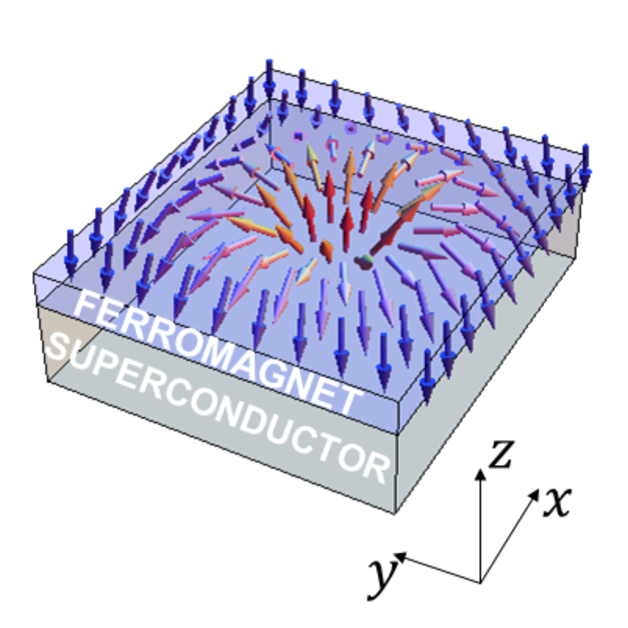
\includegraphics[width=0.4\linewidth]{SkyrmA}
(b) 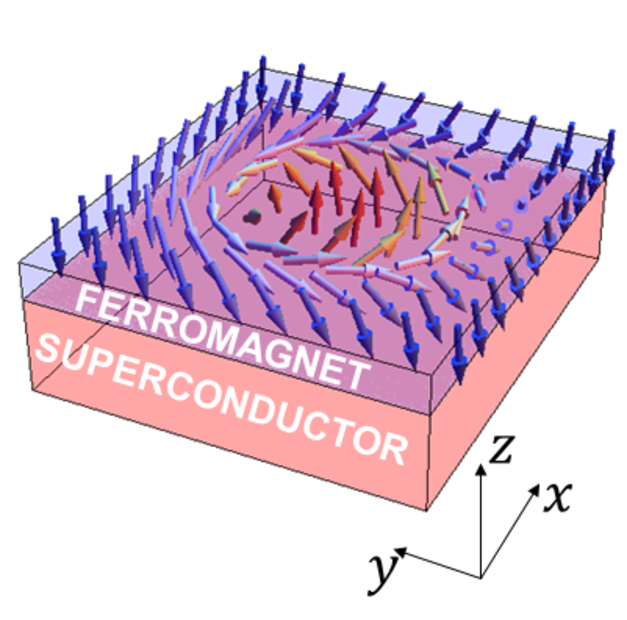
\includegraphics[width=0.4\linewidth]{SkyrmB}
\caption{(Color online.) Ferrormagnetic film deposited on top of a superconductor. The ferromagnetic vector has skyrmion configuration. (a) Hedgehog skyrmion.  (b) Spiral skyrmion. } \label{fig:skyrmion}
\end{figure}
%%%%%%%%%%%%%%%%%%%%%%%%%%%%%%%%%%%%%%%%%%%%%%%%%%%%%%%%%%%%%%%%%%%%%%%%%%


%%%%%%%%%%%%%%%%%%%%%%%%%%%%%%%%%%%%%%%%%%%%%%%%%%%%%%%%%%%%%%%%%%%%%%%%%%%
\begin{figure*} \centering
	(a)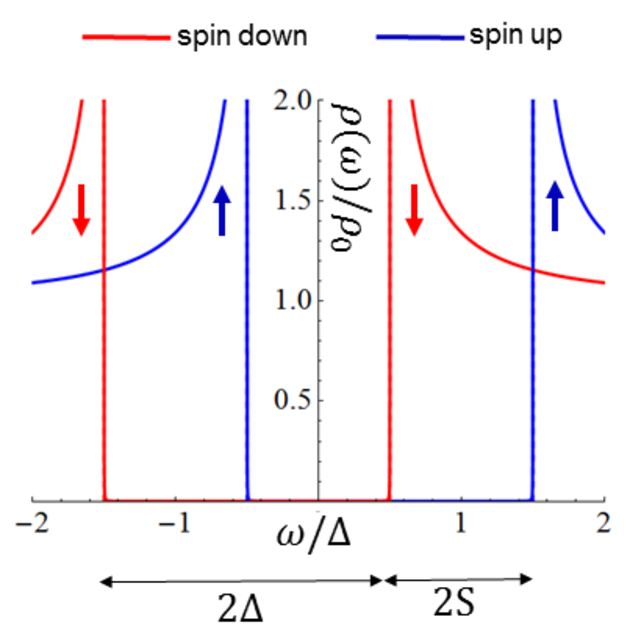
\includegraphics[width=0.25\linewidth]{LDOSa} \hspace{0.1cm}
	(b)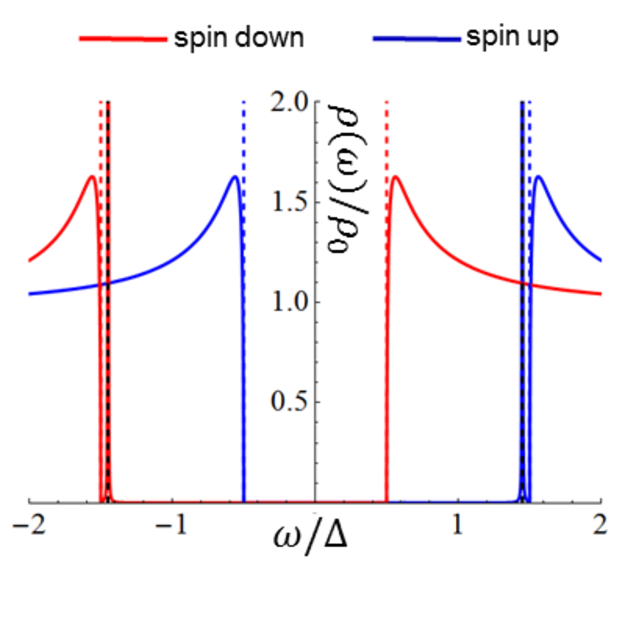
\includegraphics[width=0.25\linewidth]{LDOSb} \hspace{0.1cm}
	(c)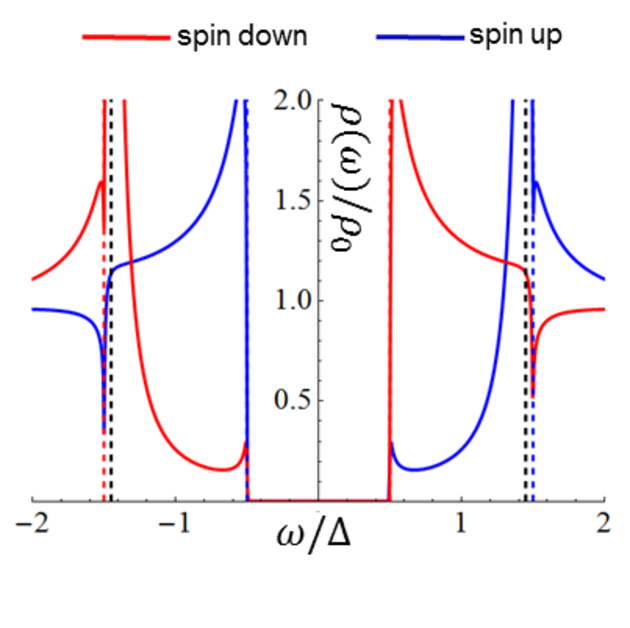
\includegraphics[width=0.25\linewidth]{LDOSc}
\caption{(Color online) Spin-polarized local density of states (a) away from the skyrmion and (b,c) at the core of the skyrmion. Panel (b) corresponds to the usual T-matrix that takes into account only out-of-plane. Panel (c) corresponds to the T-matrix that takes into account in-plane spin. Comparing (b) and (c) notice that a thin YSR state in (b) becomes a thick resonance in (c). The parameters of plots are $2S = \Delta = 0.25 E_F$ and $R = 1/p_F = \xi/8$. Blue and red dashed lines indicate the positions of the shifted spin-up and spin-down bands, respectively. The black dashed line indicates the position of the YSR pole, given by Eq.~.} \label{fig:LDOS}
\end{figure*}
%%%%%%%%%%%%%%%%%%%%%%%%%%%%%%%%%%%%%%%%%%%%%%%%%%%%%%%%%%%%%%%%%%%%%%%%%%


Let the three-dimensional vector $S(\bm r) = (S_x,S_y,S_z)$ describe the configuration of the ferromagnetic vector in a two-dimensional ferromagnetic film $\bm r = (x,y)$. The configurations of the field $S(\bm r)$ shown in Fig.~\ref{fig:skyrmion}(a) and (b) are referred to as skyrmions. The skyrmion configuration of the field is characterized by the topological charge

\begin{align}
	Q = \frac{1}{4\pi} \int d^2r \, \hat {\bm S}\cdot (\nabla_x\hat {\bm S}\times\nabla_y\hat {\bm S}), \quad \hat {\bm S}= \frac{\bm S}{S},
	\label{topCharge}
\end{align}
which cannot be altered by the continuous transfomation of the field.  We also characterize the skyrmion fields by the zeroth and first moments
\begin{align}
	S^{(0)}_i = \int  d^2r \, \left[S_i(\bm r)-S_i(\infty)\right],\,\, i\in \{x,y,z\}, \label{S0} \\
	S^{(1)}_{ij} = \int  d^2r \, \left[S_i(\bm r)-S_i(\infty)\right] r_j,\,\, j\in \{x,y\}. \label{S1}
\end{align}
The zeroth moment $\bm S^{(0)} = S_{\rm e} \hat{\bm z}$ characterizes the effective out-of-plane magnetic moment of the skyrmion and is equal for the two skyrmions shown in Fig.~{\ref{fig:skyrmion}}(a) and (b). Whereas, the first-order moment $S^{(1)}_{ij}$ characterizes the in-plane pattern of the ferromagnetic vector $\bm S(\bm r)$. Note that for the cylindrically symmetric field $S(\bm r)$, the first order moment defined in Eq.~(\ref{S1}) can be expanded in the symmetric and antisymmetric parts
\begin{equation}
	S^{(1)}_{ij}=S_{\rm m}\,\delta_{ij} + S_{\rm a}\,\epsilon_{ijz}
\end{equation}
The skyrmions shown in Fig.~\ref{fig:skyrmion}(a) and (b) have monopole $S_{\rm m}$ and anapole $S_{\rm a}$ moments correspondingly, hence the name of the skyrmions. However the two types of the skyrmions have the same topological charge~(\ref{topCharge}) and can be continuosly deformed into each other.

%%%%%%%%%%%%%%%%%%%%%%%%%%%%%%%%%%%%%%%%%%%%%%%%%%%%%%%%%%%%%%%%%%%%%%%%%%%
\begin{figure*} \centering
	(a)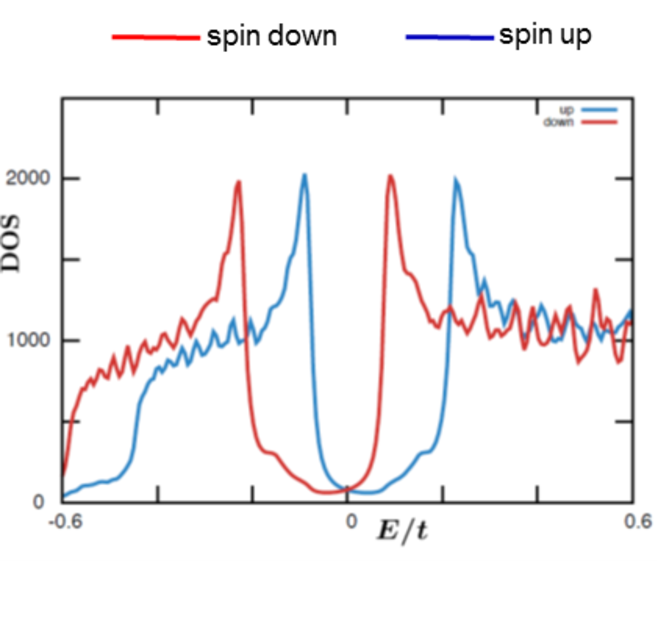
\includegraphics[width=0.25\linewidth]{numerical-LDOS-away} \hspace{0.1cm}
	(b)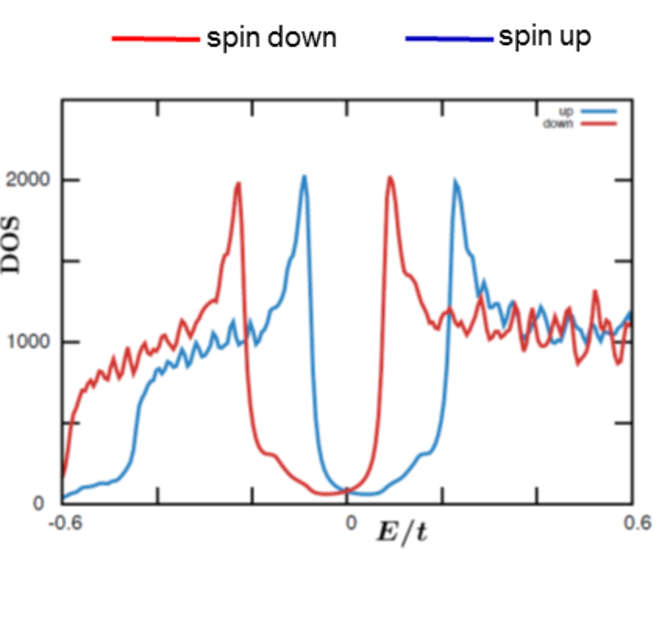
\includegraphics[width=0.25\linewidth]{numerical-LDOS-core} \hspace{0.1cm}
	(c)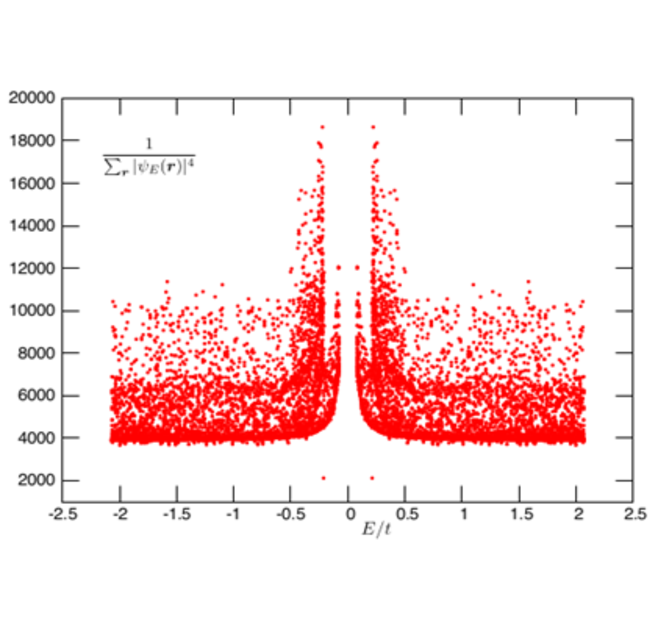
\includegraphics[width=0.25\linewidth]{numerical-IPR}
\caption{(Color online) Numerical modeling of a skyrmion: (a) LDOS away from the skyrmion (PLEASE SUBSTITUTE WITH THE CORRECT FIGURE), (b) LDOS at the skyrmion core, (c) inverse participation ratio (IPR).} \label{fig:LDOSNumerics}
\end{figure*}
%%%%%%%%%%%%%%%%%%%%%%%%%%%%%%%%%%%%%%%%%%%%%%%%%%%%%%%%%%%%%%%%%%%%%%%%%%

%%%%%%%%%%%%%%%%%%%%%%%%%%%%%%%%%%%%%%%%%%%%%%%%%%%%%%%%%%%%%%%%%%%%%%%%%%%
\paragraph*{Model}  \label{sec:model}
%%%%%%%%%%%%%%%%%%%%%%%%%%%%%%%%%%%%%%%%%%%%%%%%%%%%%%%%%%%%%%%%%%%%%%%%%%
The model is given by the following Hamiltonian
=======
The model is given by the following 4-by-4 Bogolyubov-de Gennes (BdG) Hamiltonian
\begin{align}
	 H &= \xi(\bm p)\tau_z+\Delta \tau_x - \bm S(\bm r)\cdot\bm\sigma, \label{ham} \\
  & \xi(\bm p) = \frac{p^2}{2m}-\mu,\quad \bm p = -i(\nabla_x,\nabla_y),
\end{align}
which describes the proximity coupling of the ferromagnetic vector $S(\bm r)$ to the itinerant electrons of a two-dimensional (2D) superconductor with the superconducting gap $\Delta$. The Pauli matrices $\bm \tau$ and $\bm \sigma$ act, respectively, in the particle-hole and spin subspaces of the four-component spinor $\Psi = (\psi_\uparrow,\psi_\downarrow,\psi^\dagger_\downarrow,-\psi^\dagger_\uparrow)^T$. For simplicity, we assume that the magnitude of the superconductor-ferromagnet coupling is constant and only the direction $\bm S(\bm r)$ varies, i.e., we set $\bm S(\bm r) = S\,\bm n(\bm r)$, where $\bm n$ is a unit vector. In order to proceed further let compare the typical lengthscales. The radius of skyrmions $R$ found in experiments~\cite{Heinze2011,Romming2013,Bergmann2014,Brede2014,Sonntag2014,vonBergmann2015,Romming2015} does not typically exceed $5$ nm, whereas the superconducting coherence length $\xi_{sc}$ varies largely from a micron to a few nanometers as in, e.g., curprates. For the analysis below, we assume the superconducting coherence length much larger $\xi_{sc}\gg R$, and briefly comment about the opposite limit in the Supplemental Material (Shall we discuss this? Local gauge transform and introduce effective spin-orbit, etc. ). In the chosen limit the superconductivity cannot ``resolve'' the fine details of the field $\bm S(\bm r)$ and only ``sees'' as a skyrmion as local magnetic defect. Therefore we shall apply a Yu-Shiba-Rusinov \cite{Yu,Shiba,Rusinov,Balatsky2006} treatment the skyrmion as a local impurity.
%%%%%%%%%%%%%%%%%%%%%%%%%%%%%%%%%%%%%%%%%%%%%%%%%%%%%%%%%%%%%%%%%%%%%%%%%%%
\paragraph*{T-matrix analysis} \label{sec:analytics}
%%%%%%%%%%%%%%%%%%%%%%%%%%%%%%%%%%%%%%%%%%%%%%%%%%%%%%%%%%%%%%%%%%%%%%%%%%%

%%%%%%%%%%%%%%%%%%%%%%%%%%%%%%%%%%%%%%%%%%%%%%%%%%%%%%%%%%%%%%%%%%%%%%%%%%%
\begin{figure*} \centering
	(a)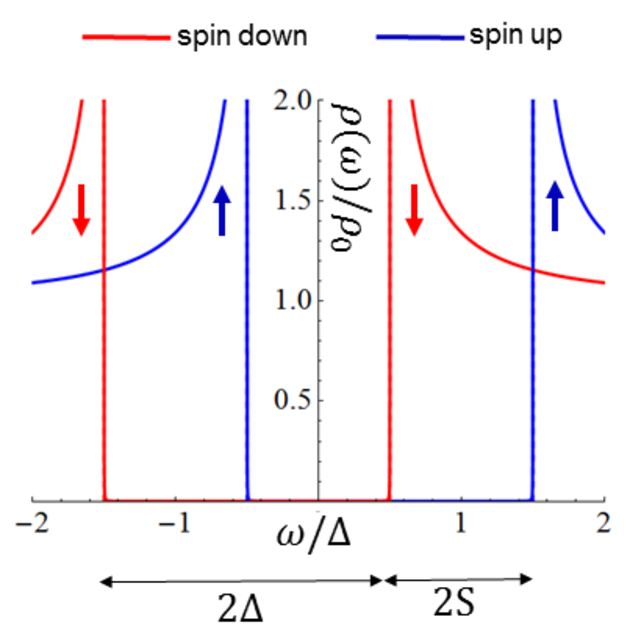
\includegraphics[width=0.25\linewidth]{LDOSa} \hspace{0.1cm}
	(b)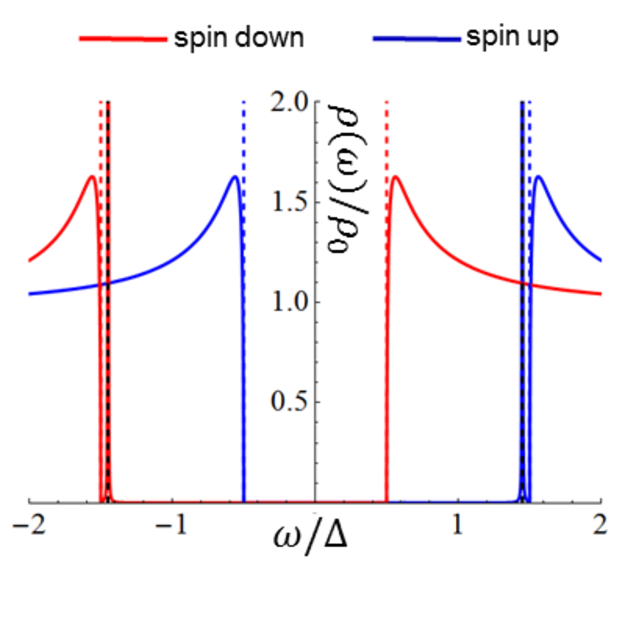
\includegraphics[width=0.25\linewidth]{LDOSb} \hspace{0.1cm}
	(c)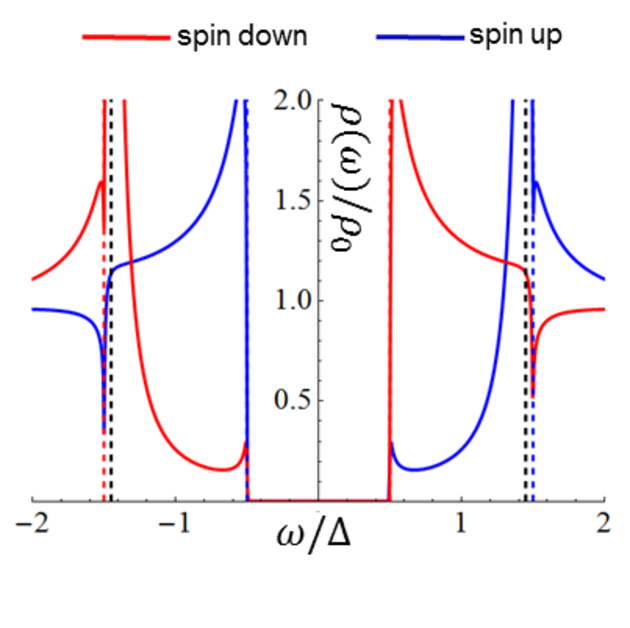
\includegraphics[width=0.25\linewidth]{LDOSc}
\caption{(Color online) Spin-polarized local density of states (SP-LDOS) away from the skyrmion (a) and at the core of the skyrmion (b,c). Panel (b) corresponds to the usual T-matrix that takes into account only out-of-plane. Panel (c) corresponds to the T-matrix that takes into account in-plane spin. Comparing (b) and (c) notice that a thin YSR state in (b) becomes a thick resonance in (c). The parameters of plots are $2S = \Delta = 0.25 E_F$ and $R = 1/p_F = \xi/8$. } \label{fig:LDOS}
\end{figure*}
%%%%%%%%%%%%%%%%%%%%%%%%%%%%%%%%%%%%%%%%%%%%%%%%%%%%%%%%%%%%%%%%%%%%%%%%%%


Superconductor-ferromagnet heterostructures were recently proposed as a viable platform for realizing topological superconductivity (TS) \cite{Lutchyn2010,Oreg2010, Sau2010}, which can host Majorana fermion quasiparticles at vortex cores and boundaries \cite{Kitaev2001, Alicea, Beenakker2013}. Majorana fermions obey non-Abelian statistics and may be utilized for topological quantum computation \cite{Read2000, Ivanov2001, Nayak2008}.  The key ingredients driving these systems in the topologically non-trivial regime are the spin-orbit coupling (SOC) and magnetism. Recently, the search for experimental realizations of TS has also led to engineering the impurity bands of the Yu-Shiba-Rusinov (YSR) states \cite{Yu,Shiba,Rusinov}, induced by magnetic atoms on the surface of a superconductor \cite{Choy2011, Nadj-Perge2013, Klinovaja2013, Vazifeh2013, Braunecker2013, Pientka2013, Nakosai2013, Poyhonen2014, Reis2014, Brydon2015, Rontynen2014, Li2015}. Following this recipe, zero-energy peaks in the tunneling spectrum were recently measured at the ends of a one-dimensional (1D) chain of magnetic atoms \cite{Yazdani2014}. Such a tunneling spectrum could be the evidence of Majorana edge states, although alternative explanations are also possible \cite{Sau2015}.


=======
It is convenient to split the Hamiltonian~(\ref{ham}) $H = h(\bm p)+V(\bm r)$ into the spatially uniform part $h(\bm p)$ and a local perturbation $V(\bm r)$ describing the skyrmion
\begin{align}
	h(\bm p) & =  \xi(\bm p)\tau_z+\Delta \tau_x - \bm S(\infty)\cdot\bm\sigma,\quad \bm S(\infty) = -S\,\hat{\bm z}\\
	V(\bm r) & =  - \left[\bm S(\bm r)-\bm S(\infty)\right]\cdot\bm\sigma  \label{vr}
\end{align}
For the skyrmions shown in Figs.~\ref{fig:skyrmion}(a) and (b), the ferromagnetic vector is $S(\infty) = -S\,\hat{\bm z}$ far from skyrmion, and is parallel to $\bm S(0)= S\hat{\bm z}$ at the skyrmion core. The Hamiltonian $h(\bm p)$ describes a superconductor proximity coupled to a ferromagnet with constant magnetization, i.e. in the absence of the skyrmion. The ferromagnetic term $S\sigma_z$ breaks two-fold Kramers degeneracy of the bands and the spectrum contains four coherence peaks with energies $\pm\Delta\pm S$ as shown in Fig.~(\ref{fig:LDOS})(a). The bands corresponding to opposite spin are decoupled. The spectrum maintains a gap as long as the Zeeman coupling is less than the superconducting gap, i.e. $S<\Delta$. Such spectrum should be possible to detect by the spin-polarized tunneling spectroscopy methods[cite relevant papers]. In the presence of the skyrmion, the term~(\ref{vr}) should be taken into account. As pointed out above, for small skyrmion size $\xi_{sc}\gg R$, the skyrmion field can be approximated as a local magnetic impurity with $V(\bm r)=S_{\rm e}\,\sigma_z \delta^2(\bm r)$\footnote{Using Eqs.~(\ref{S0}) and (\ref{S1}), the moments can be expressed via the original parameters of the model as $S_{\rm e} = c_1 S R^2$ and $S_{\rm m} = c_2 S R^3$, where $S$ is ferromagnetic coupling and $R$ - the skyrmion radius. The coefficients $c_1\approx 5.18$ and $c_2\approx 6.53$ are calculated in the Supplementary Material for a specific model. }. Such a local perturbation can be  treated exactly by calculating the T-matrix
\begin{align}
	T(\omega) =   \frac{-S_{\rm e}\sigma_z}{1+S_{\rm e}\sigma_zg_{0}(\omega)} \label{tm}
\end{align}
taken into account in T-matrix calculation, which gives the following SP-LDOS at the skyrmion core
\begin{align}
	\rho_s & (\omega) = \label{ldos} \\
	&-\frac{1}{\pi}\,{\rm Im}{\rm \,Tr} \left\{  \frac{1+\tau_z}{2}\,\frac{1+\sigma_s}{2} \left[g_0(\omega)+g_0(\omega) T(\omega) g_0(\omega)  \right]\right\},\nonumber
 \end{align}
 where energy has infinitesimally small imaginary part in the right side of the equation, i.e. $\omega\rightarrow \omega+i\delta$, and $s=x,y,z$ denotes the spin quantization axis. In Eqs.~(\ref{tm}) and (\ref{ldos}), the $g_0(\omega)$ is the on-site matrix element of the Green's function $g(\omega,\bm p) = [\omega-h(\bm p)]^{-1}$
 \begin{align}
	 g_{0}(\omega)  =-\pi\rho\sum_{\lambda = \pm 1} \frac{1+\lambda\sigma_z}{2}\,\frac{\omega-\lambda S+\Delta\tau_x}{\sqrt{\Delta^2-\left( \omega-\lambda S \right)^2}},  \label{grf}
\end{align}
where $\rho = m/2\pi$ is the density of states. We plot LDOS (\ref{ldos}) in Fig.~\ref{fig:LDOS}(b). We observe that the skyrmion-YSR (SYSR) states split from the bulk bands. The energy of the states is given by the poles of the T-matrix, i.e. satisfy the equation $1+S_{\rm e}\sigma_zg_{0}(\omega)=0$, which gives
\begin{align}
	E^\pm_{\rm SYSR} = \pm\left[S+\Delta \frac{1-\left( \pi\rho S_{\rm e} \right)^2}{1+\left( \pi\rho S_{\rm e} \right)^2}\right].
	\label{energy}
\end{align}
 The SYSR states maintain the spin polarization of the bands they split off: the positive (negative) SYSR state ``up'' (``down'') spin-polarized. For small skyrmions $R\sim 1/p_F$, the effective magnetic moment of a skyrmion $S_{\rm e}$ is small, and, so, the SYSR states are close to the outter  coherence peaks $\pm(\Delta+S)$ as seen in Fig.~\ref{fig:LDOS}(b).  Therefore the SYSR states lie inside continuum of states with the opposite spin. In the absence of coupling between the spin-``up'' and ``down'' sectors of the Hamiltonian, the SYSR states do not mix with the background delocalized states and maintain zero spectral width. In this respect, they do not differ much from the conventional YSR states.

 In such a way, we have shown that the skyrmion can be treated as a point impurity and induces a YSR-like state in the spectrum. Let us now expand the model by taking into account that the in-plane spins, which are unavoiably present around the skyrmion, can couple the up and down sectors of the Hamiltonian. As discussed above, the in-plane spins are characterized by the first moment tensor~Eq.~(\ref{S1}). In the case of the hedgehog skyrmion, the tensor only contains the diagonal component corresponding to the monopole moment $S_{\rm m}$. Therefore we modify the local perturbation describing the skyrmion as $V(\bm r) =  S_{\rm e}\, \sigma_z\delta^2(\bm r) - S_{\rm m}\, \bm\sigma\cdot\bm \nabla\delta^2(\bm r)$. We repeat the T-matrix calculation for this perturbation in the Supplementary Material and obtain
\begin{align}
	T(\omega) =   \frac{-S_{\rm e}\sigma_z+S^2_{\rm m}p_F^2\bar g_{0}(\omega)}{1+S_{\rm e}\sigma_zg_{0}(\omega)-S^2_{\rm m}p_F^2\,\bar g_{0}(\omega)\, g_{0}(\omega)}, \label{tm1}
\end{align}
where for brevity $\bar g_0(\omega) = \frac{1}{2}\sum_{j=x,y} \sigma_j g_0(\omega) \sigma_j $ is the Green's function obtained from Eq.~(\ref{grf}) by substitution $\sigma_z\rightarrow -\sigma_z$. We compare Eqs.~(\ref{tm}) and (\ref{tm1}) and observe that the latter contains renormalized numerator and the denominator due to $S_m$. We substitue the T-matrix~(\ref{tm1}) in Eq.~(\ref{ldos}) and plot LDOS in Fig.~\ref{fig:LDOS}(c). We observe the LDOS around the SYSR state has significantly widened. In order to explain this, let us consider poles of the T-matrix~(\ref{tm1}) given by $1+S_{\rm e}\sigma_zg_{0}(\omega)-S^2_{\rm m}p_F^2\,\bar g_{0}(\omega)\, g_{0}(\omega)=0$. The real part of this equation still gives the SYSR state given by Eq.~(\ref{energy}). However, since $\bar g_0(\omega)$, which is the Green's function for a flipped spin, is imaginary at the SYSR energy, the term $S^2_{\rm m}p_F^2\,\bar g_{0}(\omega)\, g_{0}(\omega)$ becomes imaginary and determines a finite spectral width of SYSR resonance. The LDOS also manifests an upshoot This explains the apparent widening of the spectrum around the SYSR state.  The LDOS even contains an upshoot around the inner coherence peaks $\pm \left( \Delta-S \right)$.
%%%%%%%%%%%%%%%%%%%%%%%%%%%%%%%%%%%%%%%%%%%%%%%%%%%%%%%%%%%%%%%%%%%%%%%%%%%
\paragraph*{Numerical analysis.} \label{sec:numerics}
%%%%%%%%%%%%%%%%%%%%%%%%%%%%%%%%%%%%%%%%%%%%%%%%%%%%%%%%%%%%%%%%%%%%%%%%%%%

Briefly introduce the model and the results. Compare to analytics. Discuss what is IPR and that it shows only a single quasi localized state. Show IPR for a smaller window of energies, e.g. $-2\Delta<\omega<2\Delta$. Does the IPR figure correspond to the LDOS figures, or is it plotted for different parameters.

%%%%%%%%%%%%%%%%%%%%%%%%%%%%%%%%%%%%%%%%%%%%%%%%%%%%%%%%%%%%%%%%%%%%%%%%%%%
\paragraph*{Long-range wave function} \label{sec:wavefuncion}
%%%%%%%%%%%%%%%%%%%%%%%%%%%%%%%%%%%%%%%%%%%%%%%%%%%%%%%%%%%%%%%%%%%%%%%%%%%
The




%%%%%%%%%%%%%%%%%%%%%%%%%%%%%%%%%%%%%%%%%%%%%%%%%%%%%%%%%%%%%%%%%%%%%%%%%%%
\paragraph*{Discussion [Comment: here we discuss importance. Long-range interactions between skyrmions mediated by superconductivity. ] } \label{sec:discussion}
%%%%%%%%%%%%%%%%%%%%%%%%%%%%%%%%%%%%%%%%%%%%%%%%%%%%%%%%%%%%%%%%%%%%%%%%%%%
\begin{figure} \centering
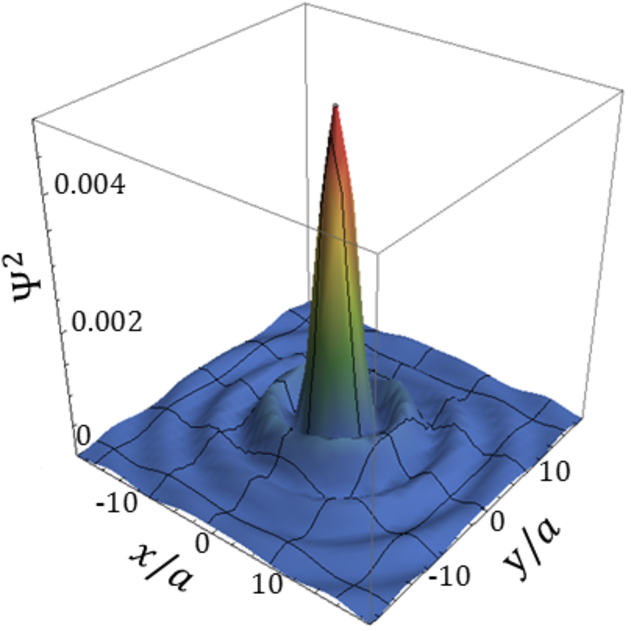
\includegraphics[width=0.7\linewidth]{WaveFunction}
\caption{(Color online) Numerical wavefunction corresponding to the sYSR state. The wave function has pronounced oscillations with a period of approximately the superconducting coherence length. [parameters for which the figures are plotted]  } \label{fig:wavefunction}
\end{figure}
%%%%%%%%%%%%%%%%%%%%%%%%%%%%%%%%%%%%%%%%%%%%%%%%%%%%%%%%%%%%%%%%%%%%%%%%%%




%%%%%%%%%%%%%%%%%%%%%%%%%%%%%%%%%%%%%%%%%%%%%%%%%%%%%%%%%%%%%%%%%%%%%%%%%%%
\paragraph*{Conclusion} \label{sec:conclusion}
%%%%%%%%%%%%%%%%%%%%%%%%%%%%%%%%%%%%%%%%%%%%%%%%%%%%%%%%%%%%%%%%%%%%%%%%%%%

There are two effects: local scattering and Zeeman field hence the DOS will be split etc.  Draw similarities and differences with single imp.
In parallel with skyrmion discovery the local imaging using magnetic probes like MFM and SP-STM allowed one to image the matter at atomic resolution while also resolving spin content of electron carriers in the substrate.
Here we prove the existence of the new type of localized excitation on the skyrmion core we call  Sc-YSR state (alternative is skyrmion bound state (sbs)).  Show the main results upfront in the introduction. Both LDOS and SP-LDOS.




%%%%%%%%%%%%%%%%%%%%%%%%%%%%%%%%%%%%%%%%%%%%%%%%%%%%%%%%%%%%%%%%%%%%%%%%%%%%%
%\bibliographystyle{apsrev4-1}
\bibliography{Skyrmion}
%%%%%%%%%%%%%%%%%%%%%%%%%%%%%%%%%%%%%%%%%%%%%%%%%%%%%%%%%%%%%%%%%%%%%%%%%%%%%


\appendix

%%%%%%%%%%%%%%%%%%%%%%%%%%%%%%%%%%%%%%%%%%%%%%%%%%%%%%%%%%%%%%%%%%%%%%%%%%%%%
\section{T-matrix analysis} \label{sec:appendixTMatrix}
%%%%%%%%%%%%%%%%%%%%%%%%%%%%%%%%%%%%%%%%%%%%%%%%%%%%%%%%%%%%%%%%%%%%%%%%%%%%%
In this section, we give an analytic treatment of the skyrmion-induced bound states using the T-matrix approximation. Starting from the Hamiltonian (\ref{ham}) in the second-quantized form, we write the Bogolyubov-de Gennes (BdG) Hamiltonian as
=======

In this section, we give an analytic treatment of the skyrmion-induced bound states using the T-matrix approximation. Starting from the Hamiltonian (\ref{ham}) in the second-quantized form, we write the Bogolyubov-de Gennes (BdG) Hamiltonian as
\begin{align}
	& H_{\rm BdG} = H(\bm p) + V(\bm r),\quad {\rm where} \nonumber \\
& H(\bm p) = \xi(\bm p)\tau_z+\Delta \tau_x - \bm S(\infty)\cdot\bm\sigma,\quad \bm S(\infty) = -S\,\hat{\bm z}, \nonumber\\
& V(\bm r) = -\left[ \bm S(\bm r)-\bm S(\infty)\right]\cdot\bm\sigma \label{v0}
\end{align}
The momentum-dependent part $H(\bm p)$ describes a superconductor coupled to a spatially uniform ferromagnetic vector $\bm S(\infty)$, whereas the position-dependent piece $V(\bm r)$ describes the local perturbation due to the skyrmion. Although the specific model is not significant, we assume the following model for the skyrmion centered at the origin $r=0$
\begin{align}
	\bm S(\bm r) &= S\left[ \cos\phi(\bm r) \sin\theta(\bm r),\, \sin\phi(\bm r)\sin\theta(\bm r),\,\cos\theta(\bm r)\right], \nonumber \\
	\phi(\bm r) &= \arctan(x/y),\quad \theta(\bm r) = \pi \left[ 1-\exp\left( -\frac{r^2}{R^2} \right) \right], 	\label{sr}
\end{align}
where $\phi(\bm r)$ and $\theta(\bm r)$ denote the polar and azimuthal angle of the vector $\bm S(\bm r)$, and $R$ controls the skyrmion size. The superconducting coherence length is usually greater than a typical skyrmion size $R\sim 5$\,nm \cite{Heinze2011,Romming2013,Bergmann2014,Brede2014,Sonntag2014,vonBergmann2015,Romming2015}, i.e. $\xi_{\rm sc}\gg R$. Therefore, the superconductivity does not ``resolve'' the fine details of the skyrmionic configuration of the field  $\bm S(\bm r)$, but rather ``sees'' its long-wavelength characteristics such as the moments described by Eqs.~(\ref{S0}) and (\ref{S1}). Motivated by this logic, we substitute the original skyrmionic field $\bm S(\bm r)$ by its local version
\begin{equation}
	\bm S(\bm r) - \bm S(\infty) = \left[ S_{\rm e}\, \hat{\bm z} - S_{\rm m}\, \bm \nabla\right] \delta^2(\bm r).
	\label{S}
\end{equation}
Here, in order to relate the moments to the original parameters of the model we subtitute Eq.~(\ref{sr}) in Eqs. (\ref{S0}) and (\ref{S1}) and find
\begin{align}
	S_{\rm e} &= SR^2 \pi  \left [-\text{Ci}(\pi )+\gamma +\log (\pi )\right] \approx 5.18\, SR^2, \\
	S_{\rm m} &= SR^3 \int_0^{\infty } 2 \pi  t^2 \sin \left(\pi  e^{-t^2}\right) \, dt \approx 6.53\, SR^3.
\end{align}
Equation  (\ref{S}) is convenient for the T-matrix calculation, which we now proceed to. We take into account (\ref{S}) and calculate the Fourier transform of Eq.~(\ref{v0})
\begin{equation}
	V(\bm p) = -S_{\rm e}\,\sigma_z +  i \,S_{\rm m} \, \bm \sigma\cdot \bm  p,
	\label{vp}
\end{equation}
using which we write an intergal equation for the T-matrix
\begin{align}
	T\left(\bm p^{1},\bm p^{2}\right) &= V \left(\bm p^{1}-\bm p^{2}\right) \nonumber \\
	& +\int d^2 p'\, V\left(\bm p^{1}-\bm p'\right) g(\omega,\bm p')  T\left(\bm p',\bm p^{2}\right).
	\label{integEq}
\end{align}
Here, the bare Green's function of the superconductor is defined as
\begin{align}
	g(\omega,\bm p) = \frac{1}{\omega-H(\bm p)} = \frac{1}{\omega-\xi(\bm p)\tau_z-\Delta \tau_x - S\sigma_z}.
\end{align}
Since in the case of the superconductivity we are interested in the scatterings close to the Fermi surface, we use $\bm p^{1} = p_F\, \bm n^{1}$ and $\bm p^{2} = p_F \,\bm n^{2}$, where the in-plane unit vectors $\bm n^{1}$ and $\bm n^{2}$ determine the direction of scattering on the Fermi surface.  Then, we seek the T-matrix in the following form
\begin{align}
	T\left(\bm n^{1},\bm n^{2}\right) &= A + B_i n^{1}_i + C_i n^{2}_j + D_{ij} n^{1}_i n^{2}_j, \label{ansatz}
\end{align}
where  $A,B_i,C_i$ and $D_{ij}$ are the matrices in the four-components space $\sigma\otimes\tau$. We substitute ansatz~(\ref{ansatz}) in the integral Eq.~(\ref{integEq}) and find the T-matrix
\begin{widetext}
\begin{equation}
	T\left(\bm n^{1},\bm n^{2}\right) = \frac{-S_{\rm e}\sigma_z+S^2_{\rm m}p_F^2\bar g_{0}(\omega)+i\,S_{\rm m}\,p_F \,  \bm \sigma\cdot(\bm n^{2}- \bm n^{1}) +S^2_{\rm m}\, p^2_F \, \bar g_{0}(\omega)\,\left(\bm \sigma\cdot\bm n^{2}\right)\,\left(\bm \sigma\cdot \bm n^{1}\right)}{1+S_{\rm e}\sigma_zg_{00}-S^2_{\rm m}p_F^2\,\bar g_{0}(\omega)\, g_{0}(\omega)},
\end{equation}
\end{widetext}
where the Green's function in the real space was denoted as
=======
where the Green's function on-site matrix element in the real space is denoted as
\begin{align}
	g_{0}(\omega) &   =\int d^2 p\, g(\omega,\bm p)  	\label{g0} \\
	 & =-\pi\rho\sum_{\lambda = \pm 1} \frac{1+\lambda\sigma_z}{2}\,\frac{\omega-\lambda S+\Delta\tau_x}{\sqrt{\Delta^2-\left( \omega-\lambda S \right)^2}}, \nonumber \\
	 \bar g_{0}(\omega) & = \frac{1}{2} \sum_{j=x,y}\sigma_j\, g_{0}(\omega)\, \sigma_j.\label{bg0}
\end{align}
For brevity, $\bar g_{0}$ denotes the Green's function obtained from $g_{00}$ by replacing $\sigma_z \rightarrow - \sigma_z$ according to Eq.~(\ref{bg0}). The density of states per spin is denoted as $\rho = m/2\pi$.
%%%%%%%%%%%%%%%%%%%%%%%%%%%%%%%%%%%%%%%%%%%%%%%%%%%%%%%%%%%%%%%%%%%%%%%%%%%%%
\subsection{LDOS} \label{sec:LDOS}
%%%%%%%%%%%%%%%%%%%%%%%%%%%%%%%%%%%%%%%%%%%%%%%%%%%%%%%%%%%%%%%%%%%%%%%%%%%%%
So, in the presence of the skyrmion, the Green's function becomes
\begin{align}
	G(\omega,\bm p^1,\bm p^2) =& g(\omega,\bm p^1)\,(2\pi)^2\delta(\bm p^1-\bm p^2) \nonumber \\
	          &  +g(\omega,\bm p^1) T(\bm p^1,\bm p^2) g(\omega,\bm p^2),
	\label{G}
\end{align}
using which the spin-polarized local density of states (LDOS) can be expressed
\begin{align}
	\rho_s(\omega,\bm r) = -&\frac{1}{\pi}\,{\rm Im}\lim_{\omega\rightarrow \omega+i\delta}{\rm\,Tr} \left[ \frac{1+\tau_z}{2}\,\frac{1+\sigma_s}{2} \right. \label{rhor} \\
	&\left.\int \frac{d^2p^1\,d^2p^2}{\left( 2\pi \right)^4} e^{i\left( \bm p^1-\bm p^2 \right)\bm r} G(\omega,\bm p^1,\bm p^2)\right]\, \nonumber
\end{align}
where $s=x,y,z$ denotes the spin quantization axis. It can be easily evaluated for instance at the skyrmion core, i.e., at $\bm r=0$,
\begin{align}
	& \rho_s(\omega,0) = -\frac{1}{\pi}\,{\rm Im}\lim_{\omega\rightarrow \omega+i\delta}{\rm \,Tr} \left\{  \frac{1+\tau_z}{2}\,\frac{1+\sigma_s}{2}  \right. \label{spldos} \\
	&\left.\left[g_0(\omega)+g_0(\omega)  \frac{-S_{\rm e}\sigma_z+S^2_{\rm m}p_F^2\bar g_{0}(\omega)}{1+S_{\rm e}\sigma_zg_{00}-S^2_{\rm m}p_F^2\,\bar g_{0}(\omega)\, g_{0}(\omega)} g_0(\omega)  \right]\right\}\, \nonumber
\end{align}

%%%%%%%%%%%%%%%%%%%%%%%%%%%%%%%%%%%%%%%%%%%%%%%%%%%%%%%%%%%%%%%%%%%%%%%%%%%
\begin{figure*} \centering
	(a)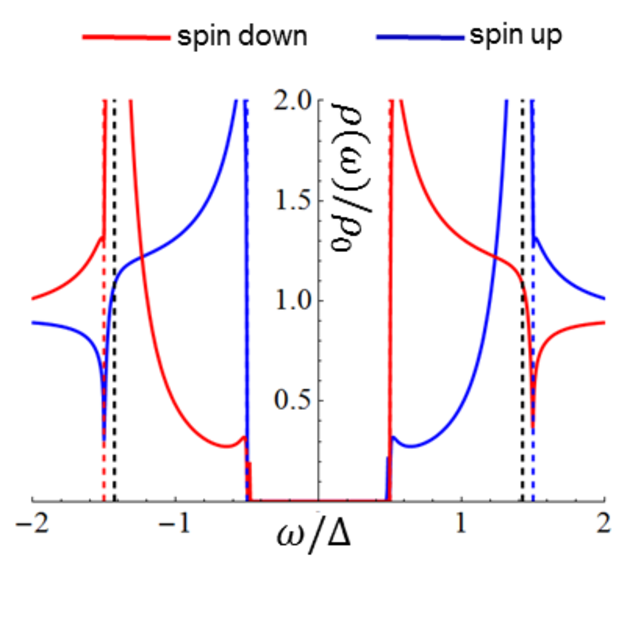
\includegraphics[width=0.25\linewidth]{ApLDOSa} \hspace{0.1cm}
	(b)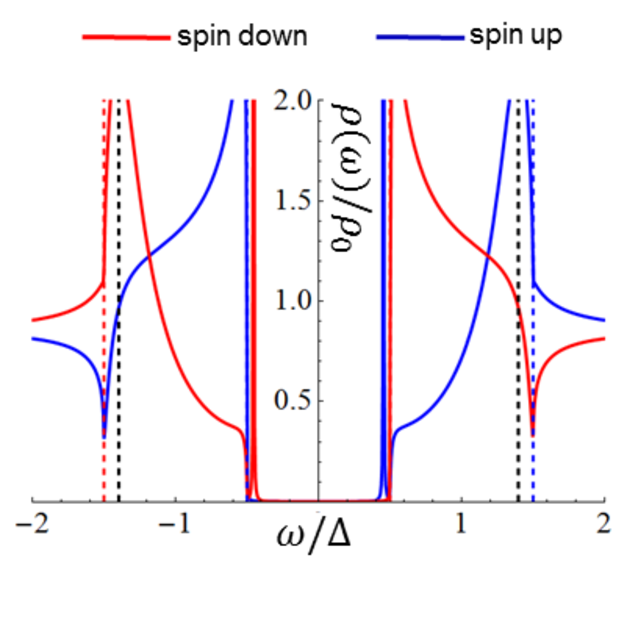
\includegraphics[width=0.25\linewidth]{ApLDOSb} \hspace{0.1cm}
	(c)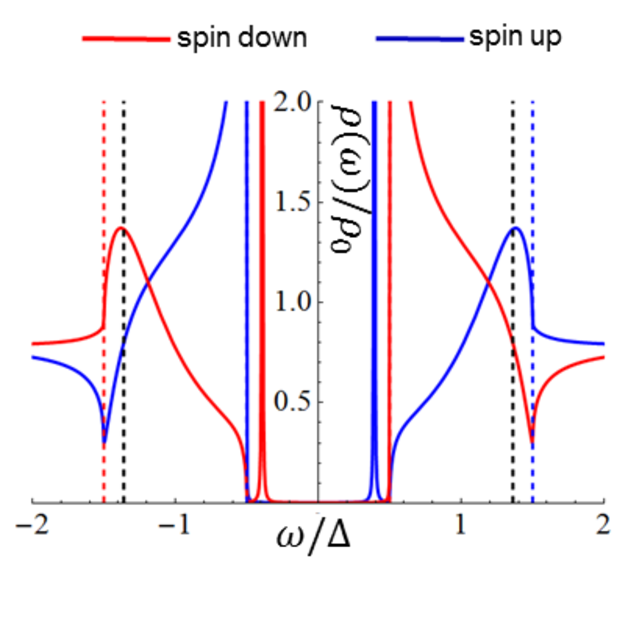
\includegraphics[width=0.25\linewidth]{ApLDOSc}
	\caption{(Color online) Spin-polarized local density of states (SP-LDOS)  at the core of the skyrmion. The consequent panels correspond to increasing skyrmion size (a) $R = 1.1 p_F^{-1}$, (b) $R = 1.2 p_F^{-1}$, (c) $R = 1.3 p_F^{-1}$. Other parameters are the same as in Fig.~\ref{fig:LDOS}. } \label{fig:ApLDOS}
\end{figure*}
%%%%%%%%%%%%%%%%%%%%%%%%%%%%%%%%%%%%%%%%%%%%%%%%%%%%%%%%%%%%%%%%%%%%%%%%%%

%%%%%%%%%%%%%%%%%%%%%%%%%%%%%%%%%%%%%%%%%%%%%%%%%%%%%%%%%%%%%%%%%%%%%%%%%%%%%
\subsection{Spatial wave function} \label{sec:wf}
%%%%%%%%%%%%%%%%%%%%%%%%%%%%%%%%%%%%%%%%%%%%%%%%%%%%%%%%%%%%%%%%%%%%%%%%%%%%%




\end{document}
